\documentclass[12pt,oneside]{book}
\usepackage{geometry}
\usepackage{qtree}
\usepackage{float}
\usepackage{enumerate}
\usepackage{listings}
\usepackage{tcolorbox}
\usepackage{mdframed}
\usepackage{labyrinth}
\usepackage{caption}
\usepackage{subcaption}
\usepackage{appendix}
\usepackage{graphicx}
\graphicspath{{images/}}

\title{Book 1}
\author{I.F.}

\definecolor{darkgrey}{RGB}{32,32,32}
\definecolor{lstbg}{RGB}{252,243,207}

\lstdefinestyle{codelst} {
  language=Python,
  showspaces=false, 
  showstringspaces=false,
  frame=single,
  numbers=left,
  backgroundcolor=\color{lstbg},
  float,
  floatplacement=H 
}

\lstdefinestyle{codelst2} {
  language=Python,
  showspaces=false, 
  showstringspaces=false,
  frame=single,
  numbers=left,
  backgroundcolor=\color{lstbg}
}

\newmdenv[topline=false,rightline=false,bottomline=false]{leftborder}

\begin{document}
\maketitle
\tableofcontents{}

\chapter{Simple decisions}
\section{Finding your path}
We are starting with reviewing how you make everyday life decisions.
Let's say you want to find your class room and now you are on the street.
You can choose between two buildings: Cinema and School.

\begin{figure}[H]
\centering
\Tree [ .{\textbf{Street}}  Cinema  School ]
\end{figure}

You know that your classroom is in the school.
You have two choices and you enter the school building. Next question
you need to answer is which stair to choose -- on the left from the
entrance or on the right:

\begin{figure}[H]
\centering
\Tree[ .{\textbf{Street}}  Cinema
[ .{\textbf{School}}  {Left stair}  {Right stair} ]
]
\end{figure}

Let's say you go to the right and you and this is
your second choice. Now you need to choose the floor: 2nd or 3rd:

\begin{figure}[H]
\centering
\Tree[ .{\textbf{Street}}  Cinema
[ .{\textbf{School}}  {Left stair}
  [ .{\textbf{Right stair}} {2nd floor} {3rd floor} ]
]
]
\end{figure}

Your choice (3rd floor) brings you next set of options:
math classroom, library, chemical lab.
You choose math classroom and that is your destination.

\begin{figure}[H]
\centering
\Tree[ .{\textbf{Street}}  Cinema
[ .{\textbf{School}}  {Left stair}
  [ .{\textbf{Right stair}} {2nd floor}
    [ .{\textbf{3rd floor}} {\textbf{Math classroom}}
      Library {Chemical lab}
    ]
  ]
]
]
\caption{Path from street to classroom.}
\end{figure}

It's good to know your path in advance, but let's change the problem:
You don't know the path but you can identify the classroom
as soon as you are there. Now you have more options:

\begin{figure}[H]
\centering
\Tree[ .{Street} [ .Cinema  {Ticket \\office} ]
[ .{School}  [ .{Left stair} [ .{Basement} [ .Gym ] ] ]
  [ .{Right stair} [ .{2nd floor}  {Library} {Restroom} ]
    [ .{3rd floor} {Math classroom}
      Library {Chemical lab}
    ]
  ]
]
]
\caption{Adding choices to the path}
\end{figure}

In computer science (CS) the structure drawn on Figures 1.1 and 1.2
are called trees and
they play an important role in a number of applications.
The search in trees is one of central algorithms in building
intelligent agents that operate in known and unknown environments.

The assumption that each decision is made based
on a finite set of options (from the street you can enter school or cinema,
right stair brings you to the 2nd or 3rd floor) is a simplification,
but a powerful one. This allows,
at least in principle, to find a solution by reviewing all possible
combinations of decisions.

Our first task will be finding path to your classroom
given the tree from Figure 1.2.

\section{How to navigate a tree}

How do we navigate a tree? In other words - how do we go over
all nodes starting from the root? The answer depends on the desired order.
Let's consider the following tree:

\begin{figure}[H]
\centering
\Tree [ .1  [ .2 [ .4 7 ] [ .5 8 9 ] ]  [ .3 [ .6 10 ] ] ]
\caption{}
\end{figure}

The order of nodes can be
1, 2, 3, 4, 5, 6, 7, 8, 9, 10 or 1, 2, 4, 7, 5, 8, 9, 3, 6, 10 -- we either go layer by layer,
or left to right.
The first path is called "in breadth", the second path is "in depth".
Each path is associated with tree search algorithm
-- "depth first search (DFS)" and "breadth first search (BFS)".

We'll start with DFS and first make an obvious observation:
\textbf{a part of a tree is a tree}.
The part of the tree above is the tree:
\begin{figure}[H]
\centering
\Tree [ .2 [ .4 7 ] [ .5 8 9 ] ]
\end{figure}

This observation gives us an idea of a search.
Suppose we want to find a node
with a given name X (6 from Figure 1.3, "math classroom" from Figure 1.2).

\begin{leftborder}
\begin{enumerate}
\item We start with the root node.
\item We check the name - if the name is X we are done.
\item If it's not we are looking into the list of children.
\item If it's empty we are also done, search failed --
the tree doesn't have the node X.
\item If it's not empty we have have new tree with each children as a root.
\item For each children node perform search taking each children
node as a root for new smaller tree.
\end{enumerate}
\end{leftborder}

Let's see how it works for searching node 6 in the tree from Figure 1.3.

\begin{leftborder}
\begin{enumerate}
\item Root is 1.
\item It's not 6 and we continue with two trees - first with root node 2
and the second with root 3.
\item Node 2 is not 6. We continue with trees starting with nodes 4 and 5.
\item Node 4 is not 6 and we continue with tree starting with node 7.
\item Node 7 is not 6 and it doesn't have children.
\item We continue with root 5
\item Node 5 is not 6 and we continue with trees starting
with nodes 8 and 9.
\item Similar to node 7: 8,9 are not 6 and they don have children.
\item We continue with tree starting with node 3
\item Node 3 is not 6 and we continue with its child node which is 6.
\textbf{We are done!}
\end{enumerate}
\end{leftborder}


\section{How to describe a tree}

\begin{tcolorbox}
\textbf{Python:} 
You need to learn basic operations and collections in 
Python -- lists, dictionaries
\end{tcolorbox}

Let's see how we can
describe the tree from Figure 2. Each node has a name, for example "School"
and a list of children - ["Left stair", "Right stair"]. The list 
of children can be empty, in this case the node is called a leaf 
or a terminal node. The node without
a parent is called root node - in our case it's "Street".

Here is how we define
the upper part of the tree:

\medskip
\textbf{(Street, (Cinema,School))}
\medskip

Adding one more layer:

\medskip
\textbf{(Street, ((Cinema,(Ticket office)), (School,(Left stair, Right stair))))}
\medskip

It doesn't look convenient and transparent, adding one more layer
will make the description not readable. 
What would help is describing the tree incrementally - node by node:

Tree1 = (Left stair,[])

Tree2 = (Right stair,[]) 

Tree3 = (School,[Tree1,Tree2])

Here is what wee did: we created Tree1 as a pair of the node
name and the list of children (this list is empty, as for this example
stairs are terminal nodes -- they don't have children). 
The same is for Tree2. The list for Tree3 is not empty, it's constructed
from two previously defined trees -- we reuse trees to avoid
nested definitions. 

The remaining part of the description:

Tree4 = (Ticket office,[])

Tree5 = (Cinema,[Tree4])

Tree6 = (Street,[Tree3,Tree5])


Here is the full initialization for the tree from Figure 1.3 in Python:

\begin{lstlisting}[style=codelst,language=Python,caption={Python: tree description}]
Tree1 = ("Math classroom",[])
Tree2 = ("Library",[])
Tree3 = ("Chemical lab",[])
Tree4 = ("Library",[])
Tree5 = ("Restroom",[])
Tree6 = ("2nd floor",[Tree4,Tree5])
Tree7 = ("3rd floor",[Tree1,Tree2,Tree3])
Tree8 = ("Right stair",[Tree6,Tree7])
Tree9 = ("Basement",[])
Tree10 = ("Gym",[])
Tree11 = ("Left stair",[Tree9,Tree10])
Tree12 = ("School",[Tree8,Tree11])
Tree13 = ("Ticket office",[])
Tree14 = ("Cinema",[Tree13])
Tree15 = ("Street",[Tree12,Tree14])

print Tree15
\end{lstlisting}

The next step is to learn how to use this tree representation to navigate
a tree. Our first task is to go through all nodes and print their names.

Let's say we start from the root node. Our steps are:

\begin{leftborder}
\begin{enumerate}
\item print the name of the root node.
\item if the node doesn't have children we are done.
\item we know children nodes and we remember that each child is a root for own tree.
So we need to do 1-3) for all children.
\end{enumerate}
\end{leftborder}

\bigskip
\begin{tcolorbox}
\textbf{Assignment:} use steps 1-3) to manually reproduce 
steps of searching node 6 in
the Figure 1.3 
\end{tcolorbox}

\section{Recursion}

\begin{tcolorbox}
\textbf{Python:} 
You need to learn about functions, loops, and conditional statements.
\end{tcolorbox}

To solve our problem and print tree node names we need
to make one important observation: \textbf{a function can call itself}.
This is called \textbf{recursion} and is of particular importance in
CS, programming, linguistic. Before we go to the tree navigation,
let's look at the example traditionally used to demonstrate
the use of recursion: calculation of factorial. Factorial of a
positive integer number $n$
is denoted as $n!$ and defined as a product of all integers
from 1 to n:

$$n! = 1 \cdot 2 \cdot\dots\cdot n$$

For example:

$$3! = 1\cdot 2\cdot 3$$
$$5! = 1\cdot 2\cdot 3\cdot 4\cdot 5$$

Two observations:

\begin{leftborder}
\begin{enumerate}
\item $1! = 1$
\item $n! = n\cdot (n-1)!$ For example $5! = 5\cdot 4!$
\end{enumerate}
\end{leftborder}

Let's first imagine and then program the following function "factorial":

\begin{leftborder}
\begin{enumerate}
\item $factorial(1)$ returns $1$
\item $factorial(n)$ for $n\neq 1$ returns $n\cdot factorial(n-1)$
\end{enumerate}
\end{leftborder}

Here is the code for factorial calculation:
\begin{lstlisting}[style=codelst2,language=Python,caption={Python: factorial}]
def factorial(n):
    if n == 1: return 1
    return n * factorial(n-1)

print factorial(5)
\end{lstlisting}

\bigskip
\begin{tcolorbox}
\textbf{Assignments:}
\begin{itemize}
\item Add printing function parameter to see the order of function calls
in the recursion.
\item Write function that calculates factorials, don't use recursion.
\item Write function that print first N Fibonacci numbers. 
Fibonacci numbers $F(i)$ are given by the following
formulas:

$$F(1) = 1$$ $$F(2) = 1$$ $$F(i) = F(i-1) + F(i-2) $$

First 6 numbers are: 1, 1, 2, 3, 5, 8.
Write two versions of the function: using loops and using recursion.
\end{itemize}
\end{tcolorbox}


\section{Navigating a tree (depth first)}
Now we can solve the problem of printing node names.
Here is the Python code --
it's the implementation of items 1-3) above.

%%%%
\newpage


\begin{lstlisting}[style=codelst2,language=Python,caption={Python: printing node names (depth first)}]
def print_node_names(T):
    print T[0]
    for child in T[1]: print_node_names(child)
\end{lstlisting}

Let's look at these 3 lines of code in more details.

\begin{leftborder}
\begin{enumerate}
\item Here we are defining function of one parameter. The parameter is a tree.
\item The tree is represented by a pair and the first element T[0] of
the pair is the name. We print it.
\item The second element T[1] of the pair is the list of node's children. 
Line 3 goes over all children and calls
\lstinline{print_node_names} for each of them.
\end{enumerate}
\end{leftborder}

Now we apply this function to print all nodes of the tree we introduced above.
\bigskip
\begin{tcolorbox}
\textbf{Assignments:}
\begin{itemize}
\item Call the function \lstinline{print_node_names}
for the tree defined above. 
\item Change the function \lstinline{print_node_names}
to print nodes in the reverse order.
\end{itemize}
\end{tcolorbox}



\chapter{Labyrinths}

\section{A maze as a tree}
Let's apply tree navigation techniques to an old problem
of finding path in a maze. For the beginning we'll be assuming that
maze is known (we have full description of a maze before we start).
Here is a simple maze:

\begin{labyrinth}{3}{4}
        \h -++
\v ++-- \h ---
\v ++++ \h --+
\v +--+ \h +++
\end{labyrinth}
%\begin{labyrinth}{3}{4}
%        \h -++
%\v +-+- \h ---
%\v ++++ \h ---
%\v +--+ \h +++
%\labyrinthsolution(0,1){uurddl}
%\end{labyrinth}

Our goal is to find a path in the maze from \textbf{A} to \textbf{B}:

\begin{labyrinth}{3}{4}
        \h -++
\v ++-- \h ---
\v ++++ \h --+
\v +--+ \h +++
\putsymbol(0,4){\small{A}}
\putsymbol(3,3){\small{B}}
\end{labyrinth}

The first question we need to answer is about the maze description.
The answer comes from the following observation: every time we
make a decision navigating the maze we make it from a finite set
of choices:

\begin{labyrinth}{3}{4}
        \h -++
\v ++-- \h ---
\v ++++ \h --+
\v +--+ \h +++
\putsymbol(0,4){\small{A}}
\putsymbol(3,3){\small{B}}
\putsymbol(0,3){\small{1}}
\putsymbol(1,3){\small{2}}
\putsymbol(2,3){\small{3}}
\putsymbol(0,2){\small{4}}
\putsymbol(1,2){\small{5}}
\putsymbol(2,2){\small{6}}
\putsymbol(0,1){\small{7}}
\putsymbol(1,1){\small{8}}
\putsymbol(2,1){\small{9}}
\end{labyrinth}


When we are in location \textbf{7} we can move to location 
\textbf{8}, when in \textbf{8} we can move to \textbf{5} or \textbf{9}.
Let's enumerate all locations and list all possible moves:

$$A\rightarrow 1,\ 1\rightarrow 4,\ 
4\rightarrow 7,\ 7\rightarrow 8,\ 8\rightarrow 5\ or\ 9,
5\rightarrow 2,\ 2\rightarrow 3,\ 3\rightarrow 6\ or\ B.$$

This structure is known from the previous chapter. It's a tree:

\begin{figure}[H]
\centering
\Tree[ .\textbf{A} [ .1 [ .4 [ .7 [ .8 [ [ .5 
[ .2 [ .3 [ 6 \textbf{B} ] ] ] ] 9 ] ] ] ] ] ] 
\end{figure}

\begin{tcolorbox}
\textbf{Assignments:}
describe this tree in Python and print the path from A to B.
\end{tcolorbox}

\section{Maze descriptions}

\begin{tcolorbox}
\textbf{Python:}
You need to learn file I/O, string processing, 
and list comprehensions in Python
\end{tcolorbox}

The maze from the figure above is small and it's easy to describe it by
manually tracing all possible moves.
For bigger mazes we need an automated way of extracting trees
from schematic representations.
For the maze above this can be something like this:

\begin{lstlisting}[language=bash]
0100000
0101111
0101010
0101000
0111110
0000000
\end{lstlisting}

Zeros represent walls and ones represent paths. You may find that the
size -- number of elements -- is different. This is the cost of introducing
walls -- they have a size on the scheme. Extracting a maze from an
image file (scanned or drawn) is technically possible, but difficult.

You can define the scheme of a maze inside your Python program, but
more flexible approach is to save schemas as text files and have one
program that can work with different mazes. 
The following piece of code combines reading the file, splitting it into lines and processing lines
element by element:

\begin{lstlisting}[language=Python,style=codelst2,caption={Python: reading a maze description}]
import sys

f = open(sys.argv[1],"r")
maze = [[x=="1" for x in line] \
       for line in f.read().split("\n") \
       if len(line)>0]
f.close()

print maze
\end{lstlisting}

\section{Converting a maze to a tree. Graphs.}

Now we have a geometrical description
of a maze -- for each element we can tell if it's a path or a wall.
Let's now convert it into a tree representing a node and its children,
or in the case of maze -- an element of a path and
elements of a path on the right-left-top-bottom (if they exist).

To make the work with a maze descriptions more convenient we need to
change the way we are identifying elements of a maze. Before we
used simple enumeration -- for small 3x3 maze above we enumerated all
9 elements from 1 to 9. For a bigger maze enumeration doesn't give a
clear picture -- where, for example, is the element 134 in the 18x13 maze?
 Instead of enumeration we'll be using two numbers -- index of a line
and index of an element position in a line. Element 1 in this notation
becomes (0,0), element 8 -- (2,1). Note zero-based indices -- we'll be
following Python list indexing convention. Enumeration can be easily
restored if needed: for a position $(i,j)$ the "old" 
index is $N\cdot i+j+1$,
where $N$ is the width of a maze: $1=3*0+0+1,\ 8=3*2+1+1$.

The use of enumeration or index pairs makes tree definition 
a little simpler --
each index is unique and we don't need to preserve a path to a node to
distinguish nodes with identical names. A tree can be defined using a
dictionary mapping unique name of a node to a list of children.

The next step is to go over the maze and create the tree. We'll be
going over the maze and for each path element analyze 
surrounding elements --
for element $(i,j)$ we'll need to check elements
$(i-1,j),\ (i+1,j),\ (i,j-1), (i,j+1)$. Adding or subtracting 1
from an index may give new index outside the maze. We'll be
skipping such cases and first write function that returns True
if an index is inside the maze, and False if it's outside:

\begin{lstlisting}[language=Python,style=codelst2,caption={Python: checking index position}]
def is_inside(index,maze_width,maze_hight):
    # checking first index component
    if index[0] < 0 or index[0] >= maze_hight: return False
    # checking second index component
    if index[1] < 0 or index[1] >= maze_width: return False
    # in all other cases index is inside
    return True
\end{lstlisting}

Now we can code the loop over all elements:
\begin{lstlisting}[language=Python,style=codelst,caption={Python: creating tree from maze}]
def create_tree(maze):
    # height of the maze is the number of lines 
    # in the definition
    height = len(maze)
    # we are assuming all lines in the definition 
    # are of the same length
    width = len(maze[0])
    # we are creating empty dictionary ...
    tree = {}
    # ... and first populate it with path elements 
    # mapped to empty lists
    for i in range(height):
        for j in range(width):
            if maze[i][j]: tree[(i,j)] = []
    # now for all elements of the tree we populated
    # lists with indices of surrounding path elements:
    for e in tree:
        i,j = e[0], e[1]
        if is_inside((i-1,j),width,height): 
            if maze[i-1][j]: tree[e].append((i-1,j))
        if is_inside((i+1,j),width,height): 
            if maze[i+1][j]: tree[e].append((i+1,j))
        if is_inside((i,j-1),width,height): 
            if maze[i][j-1]: tree[e].append((i,j-1))
        if is_inside((i,j+1),width,height): 
            if maze[i][j+1]: tree[e].append((i,j+1))
    return tree

\end{lstlisting}

\begin{tcolorbox}
\textbf{Assignment:}
Combine reading a maze from a file, maze parsing,
index verification, and tree creation into one program.
Run the program and review results.
\end{tcolorbox}

As we can see the tree constructed above is different from
trees we've seen before. Note that a node contains its parent
in the list of children -- we do not distinguish
parents and children and operate only with neighbors.
This creates the following problem: the tree navigation
algorithm we used before includes the loop over all
children. If parent node in in the list of children
the loop becomes infinite, or, taking into account
that we used recursion, recursion becomes infinite.

Similar problem arises when a maze has loops.
As a result we may start going into circles:

\begin{labyrinth}{3}{4}
        \h -++
\v +-+- \h ---
\v ++++ \h ---
\v +--+ \h +++
\labyrinthsolution(0,1){uurddl}
\end{labyrinth}

The node structure doesn't form a tree. 
The structure where nodes can form loops is
called a \textbf{graph}. Tree is a graph without loops.

To navigate a graph and find a path between two nodes we
have to modify the algorithm by keeping a record of visited
nodes. Updated version of Depth First Search:

\begin{lstlisting}[language=Python,style=codelst2,caption={Python: DFS with saving visited nodes}]
def DFS(graph,node,visited):
    # adding new node to the list of visited
    visited.append(node)
    # for each node ...
    for child in graph[node]:
    # ... if it's not visitied
        if child not in visited:
            DFS(graph,child,visited)
\end{lstlisting}

Function now takes two more parameters: current node and the list
of visited nodes. When calling the function we are using
an entrance node and empty list.

\begin{tcolorbox}
\textbf{Assignment:}
Combine tree created from a maze definition with DFS function and
print all visited nodes. Use (0,1) as the entrance node.
\end{tcolorbox}

\section{Finding the exit}

We may see that \textbf{DFS} function actually doesn't do any search --
it goes over \textbf{all} nodes. That's not what we need -- the search must
stop when we come to the exit. We have to add new parameter -- \textbf{goal}
that identifies the exit node, and to check each node:

\begin{lstlisting}[language=Python,style=codelst2,caption={Python: DFS with checking the goal}]
def DFS(graph,node,visited,goal):
    visited.append(node)
    # stop if we've reached the goal
    if node == goal: return True
    for child in graph[node]:
        if child not in visited:
            # mini-assignment: why do we need this check?
            if DFS(graph,child,visitedi,goal): return True
    # we'll come here if the maze doesn't have a solution
    return False
\end{lstlisting}


\begin{tcolorbox}
\textbf{Assignment:}
Modify the code of the previous assignment and find the path from
entrance to exit.
\end{tcolorbox}


\section{Breadth first search (BFS)}

When we started talking about navigating a tree we've mentioned
two algorithms. One -- depth first search -- we've learned in
previous sections. Let's consider the second one -- breadth first
search where we go layer by layer in a tree. For general graph
BFS first examines all neighbors (children) of a node before
increasing the depth. Similar to DFS BFS is keeping track of
visited nodes to avoid going into a loop.

The algorithm includes the following steps:

\begin{enumerate}
\item For each node we need to keep path from the start.
\item We create a list \textbf{Q} that for each node we need to check
will keep a queue of pairs (path,node). In the beginning the list contains
only starting node.
\item We create an empty list \textbf{V} to keep visited nodes.
\item The main loop continues while we have nodes to visit, or
in other words -- while the queue \textbf{Q} is not empty.
\item On each step we take first element of \textbf{Q} as our
current node and remove it from the queue.
\item We stop if the current node is our goal.
\item We skip the current node if it's in \textbf{V}.
\item In all other cases we append current node to \textbf{V} and
path and all neighbors of the current node to \textbf{Q}.
\item We continue the main loop.
\end{enumerate}

Here is Python code:

\begin{lstlisting}[language=Python,style=codelst,caption={Python: Breadth first search}]
def BFS(graph,start,goal):
    # initializing queue
    Q = [([start],start)]
    # initalaizing list of visited nodes
    V = []
    # main loop while Q is not empty
    while len(Q)>0:
        path, current_node = Q[0]
        # remove current node from the queue
        Q = Q[1:]
        # are we done?
        if current_node == goal: return (path,True)
        # have we already been here?
        if current_node in V: continue
        # saving current node
        V.append(current_node)
        # loop over all neighbors
        for neighbor in graph[current_node]:
            Q.append((path+[neighbor],neighbor))
    # we cannot reach the goal: returning empty path
    return ([],False)
\end{lstlisting}

You can rewrite the code using more efficient Python structure \textbf{dqueue}.

\begin{tcolorbox}
\textbf{Assignments:}
\begin{enumerate}
\item compare DFS and BFS for the following maze:
\begin{labyrinth}{3}{4}
        \h -++
\v +--- \h ---
\v ++++ \h ---
\v +-++ \h +++
\end{labyrinth}
\item compare DFS and BFS for bigger maze:

\begin{lstlisting}[language=bash]
010000000000
011111111110
010000001000
010111111110
010100000010
010101111110
011100100010
010111101000
010010111110
010110000010
011100111111
000000000000
\end{lstlisting}

Create file with description of the maze, parse it into graph,
do search.
\end{enumerate}
\end{tcolorbox}


\section{Unknown maze}

In previous parts we were assuming that we have a maze
description before we start searching. Our approach
was to create a full graph and use BFS of DFS to
find exit. What if we don't have full maze description and
all we can do is to analyze environment and distinguish
walls and paths -- we can enter a maze, look around
and list all possible moves. We can count our steps
to use (i,j) indices for elements of the maze.

For the simple maze we considered
in the beginning we don't know anything about elements
with question marks -- we know our current position (0,0)
and we see that we can move to (1,0) only.

\begin{labyrinth}{3}{4}
        \h -++
\v ++-- \h ---
\v ++++ \h --+
\v +--+ \h +++
\putsymbol(0,3){\raisebox{2pt}{\tiny{0,0}}}
\putsymbol(1,3){\raisebox{2pt}{\tiny{?}}}
\putsymbol(2,3){\raisebox{2pt}{\tiny{?}}}
\putsymbol(0,2){\raisebox{2pt}{\tiny{1,0}}}
\putsymbol(1,2){\raisebox{2pt}{\tiny{?}}}
\putsymbol(2,2){\raisebox{2pt}{\tiny{?}}}
\putsymbol(0,1){\raisebox{2pt}{\tiny{?}}}
\putsymbol(1,1){\raisebox{2pt}{\tiny{?}}}
\putsymbol(2,1){\raisebox{2pt}{\tiny{?}}}
\end{labyrinth}

When we are in (2,1) we remember our path and know that we can 
move to (2,2) and (1,1):

\begin{labyrinth}{3}{4}
        \h -++
\v ++-- \h ---
\v ++++ \h --+
\v +--+ \h +++
\putsymbol(0,3){\raisebox{2pt}{\tiny{0,0}}}
\putsymbol(1,3){\raisebox{2pt}{\tiny{?}}}
\putsymbol(2,3){\raisebox{2pt}{\tiny{?}}}
\putsymbol(0,2){\raisebox{2pt}{\tiny{1,0}}}
\putsymbol(1,2){\raisebox{2pt}{\tiny{1,1}}}
\putsymbol(2,2){\raisebox{2pt}{\tiny{?}}}
\putsymbol(0,1){\raisebox{2pt}{\tiny{2,0}}}
\putsymbol(1,1){\raisebox{2pt}{\tiny{2,1}}}
\putsymbol(2,1){\raisebox{2pt}{\tiny{2,2}}}
\end{labyrinth}


Would it be possible for us to find the path? The answer
is yes, we can find the path even if don't have full graph
in the beginning -- we can construct it when navigating the
maze, accumulating the knowledge about the operating environment.
If we look at DFS or BFS we can easily find that we don't
need information about the graph, except for the list of
already visited nodes and the list of neighbors.

Our approach will be to start with empty graph,
query environment (look around),
find neighbors and update the graph with new information.

To query environment we'll need a function that returns
all neighbors for a given (i,j) node. We've already done
this in the function converting a maze description into
a graph, only that function went over all maze elements
and now we need a smaller function for a single element.

\begin{tcolorbox}
Assignments:
\begin{enumerate}
\item Write functions that return neighbors.
\item Adjust BFS and DFS functions to navigate a maze
with unknown in the beginning graph.
\end{enumerate}
\end{tcolorbox}

\section{Loading a maze from an image}

So far we were using small mazes. They gave us some idea
how search algorithms work, but size was not big enough
to compare performance and resulting paths. It's inconvenient
to describe a big maze manually by entering 1s and 0s, so
let's load mazes from images. Here is an example of hand-drawn
maze:

\begin{center}
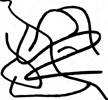
\includegraphics{maze_1s}
\end{center}

You can use a drawing program (PaintBrush or an equivalent),
or draw a maze on paper and then scan or make a picture with
a phone. Make sure lines are thick enough to avoid problems
with image resizing.

You can see an image as a list of pixels going row by row
from the top to the bottom. For a tiny image of 4 rows and
3 columns the first 3 elements of the list (list indices are 0,1,2)
describe the first row, elements with indices 3,4,5 - the second row, etc...

There is a variety of image formats and color modes. Color mode
defines the way to describe color of a pixel. Most popular mode
is RGB (red-green-blue) -- the color is defined as a combination
of three numbers representing red, green, and blue components
of a color. Each number is between 0 and 255. For example:

(0,0,0) -- black

(255,0,0) -- red

(0,255,0) -- green

(0,0,255) -- blue

(255,255,255) -- white

When all RGB components are equal the color is grey: (128,128,128),
(35,35,35), (233,233,233) are all shadows of grey. For
grey-scale images the color may be represented by a single number
between 0 and 255.

We'll not be going into pretty wide area of image processing.
For purposes of the course we need to be able to read the image
into a list of pixels, identify image height and width, 
identify dark pixels
(we'll be considering them as elements of path), change color
of a pixel to indicate found path or visited elements, and save
images into a file.

\begin{tcolorbox}
\textbf{Python:} please refer to Appendix B to learn
basics of image processing.
\end{tcolorbox}

\begin{tcolorbox}
\textbf{Assignments:}
\begin{enumerate}
\item Load maze from an image file, create a graph, find paths
using DFS and BFS.
\item Load maze from an image file, find paths and visited nodes
using both DFS and BFS \footnote{Depending on your system
settings you may get error message when doing recursive search
with DFS -- the number of recursion calls is limited to avoid
infinite recursion. If you see this problem change recursion limit
before calling DFS function: use \textbf{sys.setrecursionlimit(N)}
in Python. Experiment with N - try different values.}
\item Adjust the image file: change color
or visited nodes to green and path nodes to red. Compare results.
\end{enumerate}
\end{tcolorbox}

\section{Adding heuristics - A* search}

Both DFS and BFS can find a path in a maze if it exists.
At the same time their performance (length of the resulting
path and number of visited nodes) may not be satisfactory -- 
sometimes we have to visit all nodes to find the path.
Time and memory requirements can make the search problematic.
Can we improve the search? Given the graph of a maze
(or in more general case -- the graph of our decisions)
we may try to change the way we choose next step. In
previous studies we didn't distinguish between node neighbors --
the order in which we visited them was arbitrary, 
it didn't reflect any idea about a desired order.

Can we change the way we choose the next node to improve
performance (make a path shorter and reduce the number of
visited nodes)? The answer is positive, although the improvement
is not guaranteed -- we can introduce new algorithm that will
work better \textbf{on average}, without improving so called
\textbf{the worst case}. In other words -- it's possible to find
a case when the algorithm doesn't improve performance, but
most of the time it works better.

What would be an "improved" way of choosing next node?
We are in somewhere inside a maze and have several choices.
Intuitively we can choose a node that is closer to the exit than others --
if we know the exit is on the right we may want to move to the
right neighbor node if it's available. More accurately we
need to choose the neighbor so that the number of steps
from the beginning to the node plus our estimation of
the distance from the node to the end is minimal. The method
is called A* (A-Star). Let's try to formalize it.

First we'll need a function that returns our estimation
of the distance from a node to the goal. Given that we can move
up-down-left-right only the distance between two nodes
$(i_1,j_1)$ and $(i_2,j_2)$ can be expressed as a sum of
distances by each direction:

$$ |i_1-i_2| + |j_1-j_2| $$

or as a Python function:
\begin{lstlisting}[language=Python,style=codelst2,caption={Distance between nodes}]
def distance(node1,node2):
    return abs(node1[0]-node2[0]) + abs(node1[1]-node2[1])
\end{lstlisting}

Similar to BFS we'll keep the queue for nodes to visit, but in A*
those nodes have to be sorted based on the measure we discussed above
(number of steps from the beginning plus expected distance).
This functionality can be implemented with basic Python lists,
but more convenient is to use already available modules.
Pythons provides all we need with module \textbf{heapq}. 

Function \textbf{heappush} adds new element to the sorted queue 
preserving the order. For example adding 2 to the list of [1, 3, 4, 5]
creates new list on [1, 2, 3, 4, 5]. If element has several
components \textbf{heappush} the sort order is according to the
first component. 

Function \textbf{heappop} returns first ("smallest") element from
the queue and removes it from queue.

Queue element for A* search has to contain the following components:
\begin{enumerate}
\item number of steps from the beginning plus estimation of the deistance
to the end -- the value we'll be using to sort element (remember --
we want to prioritize nodes with smaller value).
\item number of steps from the beginning
\item path from the beginning
\item node
\end{enumerate}

\begin{lstlisting}[language=Python,style=codelst2,caption={Python: A* search}]
from heapq import heappop
from heapq import heappush

def AStar(graph,start,goal):
    Q = []
    heappush( Q, (distance(start,goal),0,[start],start) )
    V = []
    while len(Q)>0:
        dist, from_start, path, current_node = heappop(Q)
        if current_node == goal: return (path,V,True)
        if current_node in V: continue
        V.append(current_node)
        for neighbor in graph[current_node]:
            dist = distance(neighbor,goal)
            Q.append((from_start+dist,from_start+1,path+[neighbor],neighbor))
    return ([],[],False)
\end{lstlisting}

You may find that the code is pretty similar to the code of BFS.
The differences are in the components of \textbf{Q} discussed before,
and in the use of \textbf{heapq} instead of plain Python lists.

\begin{tcolorbox}
\textbf{Assignments:}
\begin{enumerate}
\item Load maze from an image file, create a graph, find paths
using A*.
\item Adjust the image file: change color
or visited nodes to green and path nodes to red. Compare results 
(paths and visited nodes) with DFS and BFS.
\item Experiment with the distance function -- try to introduce
the distance between nodes in a different way. Compare results.
\end{enumerate}
\end{tcolorbox}

\section{Challenge 1: build library of search functions and maze processing}

\begin{tcolorbox}
\textbf{Python:} please refer to Appendix to learn
module programming -- file organization and module function access.
\end{tcolorbox}

By this time you have already developed several useful functions:
\begin{enumerate}
\item Search functions: DFS, BFS, A*.
\item Maze operations: loading from a maze description, loading from an image file.
\item Creating a graph from a maze description.
\end{enumerate}

The first challenge in this course is to create Python module providing
this functionality. Keep search and maze-related functions separately.

After you are done with writing module redo your assignments using
the module. The goal is learn how to write reusable code.







\chapter{Solving puzzles}


\begin{appendices}
\chapter{Python basics}

This section covers elements of Python programming required to
complete the course. Please refer to a systematic course on Python
to learn more advanced elements of the language.

\section{Programming -- basic concepts}

Let's start with reviewing elements that don't dependent
on the programming language and then see how they work in
Python. Programs implement algorithms and
as a rule take some data as an input and generate data as an output.
Data types are domain-specific - different applications require
different data elements and
data organization, but the most common types are:

\begin{leftborder}
\begin{enumerate}
\item Logical constants: True and False.
\item Single numbers: last price on the market, number of
cars on the parking, age, number of seconds between two events,
universal constants, etc. 5, 3.1415926, 123.97.
\item Text: single characters, words, sentences, documents, text of news
\item Lists of elements: historical prices, weather records,
network traffic. Elements of lists can be accessed by their
position in the list - first element, second element, etc.
Lists are very common and fundamental in programming and in CS.
The name of one of the eldest programming languages -- LISP --
stands for LISt Processor.
\end{enumerate}
\end{leftborder}

\section{A few words on programming environments}
If Python is not installed please go to python.org and follow
instructions for your operating system.
We assume a student can create a text file with the code of the program
and execute command:

\begin{lstlisting}[language=bash,style=codelst2,caption={Python: runnning program saved in filename.py}]
python filename.py
\end{lstlisting}

Traditionally the first program is printing "Hello world!".
\footnote{Files with source codes of all examples are attached.}
Here is its listing in Python:

\begin{lstlisting}[style=codelst2, language=Python,caption={Python: Hello World!}]
print "Hello world!"
\end{lstlisting}

\bigskip
\begin{tcolorbox}
\textbf{Assignment:} create file HelloWorld.py with this program
and run in the command line:
\begin{lstlisting}[language=bash,frame=single,caption={Python: run HelloWorld.py}]
python HelloWorld.py
\end{lstlisting}
\end{tcolorbox}

\section{Basic operations}

Start Python interactive shell and enter commands (Listing A.2) one by one.

\begin{lstlisting}[style=codelst,language=Python,caption={Basic types}]
# Boolean
b = True

# Integer number
x = 2

# Float number
y = 1.23

# String
s = "Abc"

# List of numbers:
L = [1,2,3,4,5]

# print everything:
print b, x, y, s, L

# Operations:
b2 = not b
print b, b2

x2 = x * 31
print x, x2

y2 = y*y
print y, y2

s2 = s.lower()
print s, s2

L2 = L[::-1]
print L, L2

a = 2
b = "A"
print a, b
a, b = b, a
print a, b
\end{lstlisting}
Lines started with \# are comments, they are not executed.
Create file with commands and execute it. 

\section{Functions in Python}

We are using "def" to declare new function, list parameters in
parenthesis, and column ":" in the end of declaration
For example:

\begin{lstlisting}[style=codelst2,language=Python,caption={First function}]
def f(x): return x*x
\end{lstlisting}

Here we've declared function \textbf{f}. The function
 takes one parameter \textbf{x},
and returns the square of the parameter. The function
can fail if multiplication is not defined for the parameter \textbf{x} --
if it's a string for example. 

The function can have more than one line of code. We can re-write
the function from our example in the following way

\begin{lstlisting}[style=codelst2,language=Python,caption={Multi-line function}]
def f(x):
    x_squared = x*x
    return x_squared
\end{lstlisting}
Note indentation - usually it's 4 spaces. The indentation defines
the body of the function and affects "visibility" of variables. 
Consider the following code:

\begin{lstlisting}[style=codelst2,language=Python,caption={Visibility of variables}]
x = 1

def f(x):
    x2 = 2*x
    return x2

def g():
    x2 = 2*x
    return x2

print f(2)
print g()
\end{lstlisting}
First we've initialized variable \textbf{x} (line 1). Then we've
defined two functions:

\begin{enumerate}
\item \textbf{f} that takes a parameters with the same
name \textbf{x} and returns \textbf{2*x}. The variable x initialized on
the line 1 doesn't affect this function and
on the line 4 the variable \textbf{x} known to
the function f is equal 2.
\item \textbf{g} that doesn't take a parameter and returns \textbf{2*x} for
any \textbf{x} defined before the function call. In this case \textbf{g}
takes \textbf{x=1} defined on the line 1.
\end{enumerate}

Functions in Python can be nested - one function can be defined in
the body of other function:

\begin{lstlisting}[style=codelst2,language=Python,caption={Nested functions}]
x = 1

def f(x):
    x = 2*x
    def g(x):
        x = x+1
        return x
    return x + g(7)

print f(2)
\end{lstlisting}
There are three independent variables \textbf{x} here.
Note double indentation -- 8 spaces -- for the body of function \textbf{g}.

\bigskip
\begin{tcolorbox}
\textbf{Assignment:}
What are values of x when you are on the lines 1, 4, 6?
Add printing value of x in different parts of the code
to check your answer.
\end{tcolorbox}


\section{Conditions}
If you program need to change behaviour depending on some condition
you can use \textbf{if} statement.
Let's say you want to print numbers in words. On simple way of doing
this is to check the number and print accordingly.

\begin{lstlisting}[style=codelst2,language=Python,caption={Checking conditions}]
n = 1
if n = = 1:
    print "one"
elif n = = 2:
    print "two"
else:
    print "not one or two"
\end{lstlisting}
Here we are using two equality signs without spaces between 
to check the value.
\begin{itemize}
\item First we compare \textbf{n} with 1.
If n is equal to 1 we print the word "one".
\item If it's not we compare \textbf{n} with 2 (note the use of \textbf{elif} statement)
and print accordingly.
\item For all other cases (\textbf{n} is not 1 or 2) we use keyword \textbf{else}.
\end{itemize}


\section{Loops}
There exist cases when your program has to iterate over elements
of a list or a dictionary, or execute some part of a code several times
probably with different parameters. In such case we can use \textbf{for}
statement:

\begin{lstlisting}[style=codelst2,language=Python,caption="Loop"]
L = ["a", "b", "c", "def"]
for e in L:
    print e
\end{lstlisting}

Very common is the case when your program iterates over the
list elements using their indices. Index is position of an element
in the list:

\begin{lstlisting}[style=codelst2,language=Python,caption={Printing list elements by index - 1}]
L = ["a", "b", "c", "def"]
for i in range(4):
    print L[i]
\end{lstlisting}

\textbf{range(4)} is function returning list of integers from 0 to n-1.
The code above is equivalent to
\begin{lstlisting}[style=codelst2,language=Python,caption={Printing list elements by index - 2}]
L = ["a", "b", "c", "def"]
for i in [0,1,2,3]:
    print L[i]
\end{lstlisting}
Note that indices start from 0: index of the first element is 0, index of
the second element is 1, etc. For the list of N elements the index of the last element
is N-1.


\section{File input/output}

\subsection{Text files - reading/writing}

Text files of different formats -- not formated plain text,
comma-separated (CSV), JSON, XML -- are widely used for a number
of applications and we'll start with reading/writing text.

File is referenced by its name. File name may include directory name.
To start working with a file you need to open it:

\bigskip
\lstinline{f = open("filename.txt","r")}
\bigskip

Here function \textbf{open} takes two parameters - 
file name and mode of operation.
The mode \textbf{"r"} opens file for reading 
starting from the very beginning. Other modes are
\textbf{"w"} - open for writing. If file doesn't exist it'll 
be created. If file exists it'll be open as an empty one and 
existing content will be lost.
\textbf{"a"} - open for appending. If file exists it'll 
be open for writing to the end of the file.

The function \textbf{open} returns an object (variable \textbf{f}) 
used to actually read/write.

After reading/writing is done file must be closed:

\bigskip
\lstinline{f.close()}
\bigskip

Here is example:

\begin{lstlisting}[language=Python,style=codelst,caption={File operations}]
# create a file with one line of text inside:
f = open("filename.txt","w")
f.write("Hello world!")
f.close

# read the file and print its content:
f = open("filename.txt","r")
content = f.read()
f.close
print content

# append some text to the file
f = open("filename.txt","a")
f.write("Hello again")
f.close
\end{lstlisting}

\begin{tcolorbox}
\textbf{Assignments:}
experiment with opening files in different modes
and reading/writing. Be careful with modes of operation.
\end{tcolorbox}

\subsection{Command line arguments. Modules in Python.}

To open a file you need to provide a file name. This can be done
directly in the code (hardcode the name). In this case you'll need to change
your program to run for the other file. As an alternative you can
specify the name as a parameter in the command line:

\begin{lstlisting}[language=bash,frame=single]
python yourprogram.py filename.txt
\end{lstlisting}

The code above can be re-written in the following way:

\begin{lstlisting}[language=Python,style=codelst,caption={Command line parameter}]
import sys

# create a file with one line of text inside:
f = open(sys.argv[1],"w")
f.write("Hello world!")
f.close

# read the file and print its content:
f = open(sys.argv[1],"r")
content = f.read()
f.close
print content

# append some text to the file
f = open(sys.argv[1],"a")
f.write("Hello again")
f.close

\end{lstlisting}

First line contains new element: \textbf{import sys}.
Python is has a notion of a module -- the way of organizing
code. To start using a module it has to be imported.

Module \textbf{sys} provides system-level functionality.
\textbf{sys.argv} is the list of command line arguments starting
from the name of Python program file.

\begin{lstlisting}[language=Python,style=codelst2,caption={Python: print command line arguments}]
import sys

for arg in sys.argv:
    print arg
\end{lstlisting}

\begin{tcolorbox}
\textbf{Assignments:}
\begin{itemize}
\item Run the code above with different parameters.
\item Write Python program that prints itself.
\end{itemize}
\end{tcolorbox}

This code prints all parts of command line. Note that all 
parameters (elements of \textbf{sys.argv}) are strings.
To pass a numerical value you need to convert corresponding parameter:

\begin{lstlisting}[language=Python,style=codelst2,caption={Python: numbers in command line}]
import sys

x = sys.argv[1]
print x, type(x)
y = int(x)
print y, type(y)
\end{lstlisting}

Function \textbf{type} returns type of the argument --
string, integer, float, list, etc.


\section{File input/output, parsing strings}

Depending on the file format parsing its content 
may be more or less difficult.
For purposes of the course we need to parse maze descriptions 
saved in text files and convert them into trees.

Python program that reads and prints the content of the file:

%%%
\newpage

\begin{lstlisting}[language=Python,style=codelst2,caption={Reading file and printing its content}]
import sys

f = open(sys.argv[1],"r")
file_content = f.read()
f.close()

print file_content
\end{lstlisting}

First we need to split the file content into lines. Lines in files
end with invisible end-of-line (EOL) symbol or two 
symbols depending on the
operating system convention. In most of the cases
the symbol is \textbf{$\sim n$} or two symbols \textbf{$\sim r\sim n$}.
Backslash in the beginning indicates a special
kind of symbols used to format the text. The following code:

\begin{lstlisting}[language=Python,style=codelst2,caption={Splitting file into strings}]
lines = file_content.split("\n")
print lines
\end{lstlisting}

\begin{tcolorbox}
\textbf{Assignment:}
Combine two pieces of code and confirm the type of 
variable \textbf{lines} (List).
Print it element by element.
\end{tcolorbox}

Next step is to convert each line into a 
list of logical constants (True, False)
so that True corresponds to a path and False 
corresponds to a wall. For example
convert \textbf{0101010} into 
\lstinline{[False,True,False,True,False,True,False]}. One way of doing
this is to go character by character in a loop over the entire string,
compare characters with 1 and 0, and append new logical value to a list:

\begin{lstlisting}[language=Python,style=codelst2,caption={String element by element}]
line = "0101010"
num = len(line)
L = []
for i in range(num):
    is_path = line[i] == "1"
    L.append(is_path)
\end{lstlisting}
In this piece of code we first use function \textbf{len} to calculate
number of characters in the line. Next we create an empty list \textbf{L}.
We go character by character using their indices in the string
and compare them with "1". Logical variable 
\textbf{is\_path} is initialized
depending on the result of comparison with "1" and then appended to 
the list.

This way of coding is valid, but not very efficient and compact.
Instead of using loop we can use so called list comprehensions. For
a list L the following expression

\bigskip
\lstinline{[f(x) for x in L]}
\bigskip
creates a list constructed by applying 
function \textbf{f} to each element
of the list. For example:

\begin{lstlisting}[language=Python,style=codelst,caption={Python: list comprehensions}]
def f1(x):
    return x*2

def f2(x):
    return x*x

L = [1,2,3,4]
L1 = [f1(x) for x in L]
L2 = [f2(x) for x in L]
print L, L1, L2

# or the same in place:
L1 = [x*2 for x in L]
L2 = [x*x for x in L]
print L, L1, L2
\end{lstlisting}

A string in Python can be treated as a list 
(with some limitations).
The following code converts string \textbf{line} into a
list of characters it contains:

\begin{lstlisting}[language=Python,style=codelst2,caption={String to list}
line = "abc"
L = [x for x in line]
print line, L
\end{lstlisting}

Now we can rewrite the code converting string element by element into
logical variables in the following way:

\begin{lstlisting}[language=Python,style=codelst2,caption={Python: string element by element}]
line = "0101010"
L = [x=="1" for x in line]
\end{lstlisting}
Here we use in place expression \textbf{x=="1"} 
for each element of the \textbf{line}.

\section{Image processing}

To proceed you need to install Python module Pillow. Run

\begin{lstlisting}[language=bash,frame=single]
pip install Pillow
\end{lstlisting}
or refer to online documentation (python-pillow.org) for your
operating system.

Here is the Python code that loads image from attached PNG file,
prints image size and mode,
converts image into list of pixels, prints maze definition,
creates new list of pixels RGB, changes color of several pixels
to red, and creates an image for the new list and saves it.

\begin{lstlisting}[language=Python,style=codelst,caption={Python: image operations}]
from PIL import Image

img = Image.open("maze_1s.png")

imglist = list(img.getdata())

w, h = img.size

for i in range(h):
    row = ["0" if p>192 else "1" \
           for p in imglist[(i*w):((i+1)*w)]]
    print "".join(row)

new_imglist = [(x,x,x) for x in imglist]
for i in range(100):
    new_imglist[i*w+i] = (255,0,0)

new_img = Image.new("RGB",img.size)
new_img.putdata(new_imglist)

new_img.save("test.jpg")
\end{lstlisting}

Let's review the code line by line:
\begin{itemize}
\item Import support for images from PIL package.
\item Load image from PNG file. 
\item Extract pixel data and convert it into a list of pixel colors.
\item Extract image size -- width and height.
\item In the loop over each row we create and print maze description 
("0" for wall, "1" for an element of path). Original image is
in gray -- shadows of gray are coded as integers between 0 and 255.
High values correspond to light gray. Everything above 192 is considered
to be a wall, everything darker is a path.
\item Create a new list: RGB triplets representing the same colors
as in the original image (all three components -- red, green, blue --
are identical).
\item To illustrate pixel color operations we change 100 pixels on the 
diagonal -- making them red. RGB value (255,0,0) corresponds to red color.
\item Create new image object: RGB color mode and the same size as in
the original image.
\item Create image pixel data from the list of RBG triplets.
\item Save new image as JPEG file.
\end{itemize}

You can use basic image operations to illustrate differences 
between graph search algorithms.

\section{Python modules}

Modules in Python is the way to organize and reuse code.
In the simplest case module is just a Python file with
functions or other Python elements.

If file \textbf{A.py} contains the following code:

\begin{lstlisting}[language=Python,style=codelst2,caption={Python: one-file module}]
def f(x):
    print "Function f from A.py"
    return x*x
\end{lstlisting}
it can be used from other Python programs or in Python interactive 
shell:

\begin{lstlisting}[language=Python,style=codelst2,caption={Python: accessing single-file module function - 1}]
import A
print A.f(2)
\end{lstlisting}
or
\begin{lstlisting}[language=Python,style=codelst2,caption={Python: accessing single-file module function - 2}]
from A import f
print f(2)
\end{lstlisting}

Bigger projects may include multiple files. In this case
module is organized by directory -- all files are saved to
the directory and the name of the directory becomes the
name of the module. In addition to Python files with
the module-specific functions one more service file is needed:
\textbf{{\_\_}init{\_\_}.py}. The file may be empty, but normally
it contains the list of elements. Consider the following
configuration: directory \textbf{module1} containing
three files: \textbf{func1.py}, \textbf{func2.py}, 
\textbf{{\_\_}init{\_\_}.py}. The code in files:

\begin{lstlisting}[language=Python,style=codelst2,caption={Python: sample module -- file \textbf{finc1.py}}]
def f1(x):
    print "Function f1 from func1 from module1"
    return x*x

def f2(x):
    print "Function f2 from func1 from module1"
    return -x
\end{lstlisting}

\begin{lstlisting}[language=Python,style=codelst2,caption={Python: sample module -- file \textbf{finc2.py}}]
def f1(x):
    print "Function f1 from func2 from module1"
    return x*x*x

def g(x):
    print "Function g from func2 from module1"
    return x+1000
\end{lstlisting}

\begin{lstlisting}[language=Python,style=codelst2,caption={Python: sample module -- file \textbf{{\_\_}init{\_\_}.py}}]
__all__=["func1","func2"]
\end{lstlisting}

There are several ways to access functions from this module:

%%%
\newpage

\begin{lstlisting}[language=Python,style=codelst2,caption={Python: accessing module functions - 1}]
import module1.func1
import module1.func2

print module1.func1.f1(2)
print module1.func1.f2(7)
print module1.func2.f1(3)
print module1.func2.g(234)
\end{lstlisting}

\begin{lstlisting}[language=Python,style=codelst2,caption={Python: accessing module functions - 2}]
from module1 import *

print func1.f1(2)
print func1.f2(7)
print func2.f1(3)
print func2.g(234)
\end{lstlisting}

\begin{lstlisting}[language=Python,style=codelst2,caption={Python: accessing module functions - 3}]
from module1.func1 import *
from module1.func2 import f1 as f1A
from module1.func2 import g

print f1(2)
print f2(7)
print f1A(3)
print g(234)
\end{lstlisting}

\section{Random numbers}

There exist algorithms that require a random number generator.
You may want to simulate a coin toss and to generate a sequence
of 0s and 1s, or to generate a random initial state, like we did in
the section on 8-puzzle in this course. 

Python provides support for random numbers in the \textbf{random}
module. Here is the code that can be used to generate a sequence of
0s and 1s:

%%%
\newpage

\begin{lstlisting}[language=Python,style=codelst2,caption={Python: random numbers, simulating a coin toss}]
from random import randint
for i in range(10):
    print randint(0,1)
\end{lstlisting}
The function \textbf{randint(A,B)} from the module \textbf{random}
returns a random integer from A to B inclusive. If you call this
function many times each number will appear equal number of times --
the function generates numbers \textbf{uniformly distributed}.
You can adjust the code above and confirm this -- just count the number 
of 0s and 1s after 100 or 1000 calls of the function.

The other useful function from the module \textbf{random} is
\textbf{random} (function name is the same as the module name):

\begin{lstlisting}[language=Python,style=codelst2,caption={Python: random numbers in the interval (0,1)}]
from random import random
for i in range(10):
    print random()
\end{lstlisting}
The function doesn't take a parameter and returns a number between 0 and 1.
Numbers are also uniformly distributed -- if you call this function 
many times the number of cases when function returns a value in any 
interval of a given size will be the same. For example -- the number
of cases when the value is below 0.5 and above 0.5 (intervals (0,0.5)
and (0.5,1) are of equal sizes), or is in the interval (0.23,0.33) 
and (0.58,0.68).

For purposes of this course we don't need other types of 
distributions and other functions from the module.

\section{Classes}

Object-oriented programming (OOP) is one of the most powerful
and widely used programming concepts. Python supports OOP and
its core element -- the notion of classes. For purposes of this
course we'll consider just basic ideas without covering all
aspects of the concept. \footnote{
If you are familiar with OOP in other languages (similar to C++)
you'll find that implementation of classes in Python
assumes members (variables and functions) are public,
and functions are virtual.}

The idea of a class is to keep data and related functionality
together. Your program may work with objects described
by object-specific data -- for example, geometrical figures,
bank accounts, game boards, etc. Geometrical figures may be
given by a center and radius (circle) or by several sizes
(triangle, rectangle) or by position of corners (arbitrary
polygon). Bank account keeps information about the owner
(name, address, email, phone number), balance, transactions, etc.

When developing a program that works with multiple geometrical
figures we may need each figure to have a common interface
functions -- for example, the function that that returns a
position of a geometrical center, or a function that returns True
if a point is inside the figure and False otherwise. Those functions
are different for different geometrical figures and it's convenient
to isolate this functionality -- the program only "knows" that
each geometrical figure has functions \textbf{center()} and
\textbf{is\_inside(point)}.

To do this we first declare a base class common for all figures
and implementing common functionality:

\begin{lstlisting}[language=Python,style=codelst2,caption={Python: base class}]
class figure(object):
    def __init__(self,name):
        self.name = name

    def center(self):
        pass

    def is_inside(self,point):
        pass

    def __repr__(self):
        return self.name
\end{lstlisting}
Let's go line by line:

\textbf{class figure(object):}

We've declared new class \textbf{figure} extending the base class
\textbf{object}. Object is the base class for almost everything in Python
 -- integers, lists, strings, etc. are all objects. What it means --
each derived class keeps (inherits) the functionality implemented
in the base class.

\textbf{ def \_\_init\_\_(self,name):}

Function \textbf{\_\_init\_\_} is called each time we create new object.
All member functions\footnote{except static functions not covered here} have
first parameter \textbf{self} -- the reference to the constructed object.
\textbf{\_\_init\_\_} may have other parameters to initialize member variables.
Here the parameter is \textbf{name} -- the name of the figure. Base class
doesn't know anything else -- all other details will be implemented in
classes derived from \textbf{figure}.

\textbf{self.name = name}

This line initializes member variable \textbf{self.name}. If we have an
instance of this class \textbf{f} the variable \textbf{name} can be
accessed as \textbf{f.name}.
Inside the class definition the first
part of this expression (the reference to the object) is \textbf{self}
and the variable is accessed as \textbf{self.name}.

Next we declare two function -- \textbf{center} and \textbf{is\_inside}.
We are using \textbf{pass} statement
to do nothing in the base class.

\textbf{def \_\_repr\_\_(self):}

Function \textbf{\_\_repr\_\_} returns a string representation of the
object. It's called each time we print something -- Python statement
\textbf{print x} prints the string returned by \textbf{x.\_\_repr\_\_()}.
For the base class this function returns the name of the figure.


Now we want to implement a rectangle. For demonstration purposes
we'll assume the corners at points $(0,0), (w,0), (0,h), (w,h)$ --
we need only two numbers to describe any rectangle -- width \textbf{w}
and height \textbf{h}.

\begin{lstlisting}[language=Python,style=codelst2,caption={Python: derived class (rectangle)}]
class rectangle(figure):
    def __init__(self,w,h):
        figure.__init__(self,"rectangle")
        self.w = w
        self.h = h

    def center(self):
        return (self.w/2,self.h/2)

    def is_center(self,point):
        return point[0]>0 and point[0]<w and\
               point[1]>0 and point[1]<h

    def __repr__(self):
        return "{}, width={}, height={}"\
               .format(self.name,self.w,self.h)
\end{lstlisting}
Note that \textbf{\_\_init\_\_} function now has different
parameters. In the beginning it calls the corresponding function
of the base class \textbf{figure}. In this case the initialization
is trivial, but in more complicated cases the reuse may be
extremely helpful. \textbf{\_\_repr\_\_} returns the string with
name and parameters.

Here is the class implementing the same functions for circle given
by radius \textbf{r} and the position of center \textbf{c}:

\begin{lstlisting}[language=Python,style=codelst2,caption={Python: derived class (circle)}]
class circle(figure):
    def __init__(self,r,c):
        figure.__init__(self,"circle")
        self.r = r
        self.c = c

    def center(self):
        return self.c

    def is_center(self,point):
        return (point[0]-self.c[0])*(point[0]-self.c[0])+\
               (point[1]-self.c[1])*(point[1]-self.c[1]) \
               < self.r*self.r

    def __repr__(self):
        return "{}, radius={}, center={}"\
               .format(self.name,self.w,self.h)
\end{lstlisting}
Now let's learn how to use these classes:

\begin{lstlisting}[language=Python,style=codelst2,caption={Python: using classes}]
fig = figure("unknown figure")
rect = rectangle(2.0,1.0)
circ = circle(3.0, (1.0,4.0))

print type(fig), fig
print fig.ceneter(), fig.is_inside((0.0,0.0))
print type(rect), rect
print rect.ceneter(), rect.is_inside((0.5,1.2))
print type(circ), circ
print circ.ceneter(), circ.is_inside((2.0,4.0))
\end{lstlisting}
We first created three objects -- basic figure, rectangle and circle and then
called corresponding functions. The same can be done in a loop:

\begin{lstlisting}[language=Python,style=codelst2,caption={Python: using classes - 2}]
L = []
L.append( figure("unknown figure") )
L.append( rectangle(2.0,1.0) )
L.append( circle(3.0, (1.0,4.0)) )

for f in L:
    print type(f), f
    print f.ceneter(), f.is_inside((0.5,1.0))
\end{lstlisting}

This section doesn't cover all aspects of classes in Python, it
considers only very basic elements needed for the development.

\section{Saving Python structures. JSON.}

Sometimes you need to save results of calculations for future use.
Sometimes the task is simple - a number can be saved in a text file,
list of numbers may be a column in a comma-separated (CSV) file.
What if we need to save a more complex, nested structure.
Consider the following variable:

\begin{lstlisting}[language=Python,style=codelst2]
X = {}
X["abc"] = [ 1, 2, [3, [4, 6, 6]], 7, 8 ]
X["def"] = { "A":34.567, "B":98.765 }
X["ghi"] = "Sample text"
\end{lstlisting}
Each element value of this dictionary has different type -- nested list,
dictionary, string. We can introduce a custom solution for this particular
case, but it may not work for other cases. It would be convenient to have
a way to save arbitrary Python variables and then load them without
doing task-specific parsing.

The Python module \textbf{json} \footnote{JSON stands for
JavaScript Object Notation. This format is
is widely used for data exchange.}
allows to do exactly this.
Here is how we can save the variable \textbf{X} from the example above:
we import new module, create a variable, open file for writing
and save (dump) it using \textbf{json.dump} function.

%%%
\newpage

\begin{lstlisting}[language=Python,style=codelst2,caption={Python: save to JSON file}]
import json

X = {}
X["abc"] = [ 1, 2, [3, [4, 6, 6]], 7, 8 ]
X["def"] = { "A":34.567, "B":98.765 }
X["ghi"] = "Sample text"

f = open("example.json","w")
json.dump(X,f)
f.close()
\end{lstlisting}
Run this code and make sure the file is created.
Now we can load the variable:

\begin{lstlisting}[language=Python,style=codelst2,caption={Python: load from JSON file}]
import json

f = open("example.json","r")
Y = json.load(f)
f.close()

print Y
\end{lstlisting}
Try this and confirm that the variable \textbf{Y} corresponds to
\textbf{X} from the previous example.

\section{Python: machine learning libraries}

This course includes a chapter on artificial neural networks (NN).
There are several Python libraries that provide tools to configure,
train, test, and use NN: scikit-learn, Tensorflow, pybrain, Caffee
among others.
For purposes of the course we'll be using \textbf{scikit-learn}. Other
libraries and stand-alone applications are used in many different
projects and have important features but \textbf{scikit-learn} covers
very wide range of techniques and it's important to learn how
use it. \textbf{scikit-learn} is not the fastest solution, but it's
very convenient for prototyping and testing ideas. One indirect
way of using the library is reviewing its documentation -- the
table of contents can serve as a reference to many of techniques
of various complexity.

Please refer to online documentation \footnote{scikit-learn.org}
to install the library. \textbf{scikit-learn} depends on two other
libraries -- \textbf{numpy} and \textbf{scipy} -- 
they'll be installed as well.

\textbf{numpy} library provides high-performance implementation
of arrays and related functionality. In this course we'll be using
\textbf{numpy} arrays together with Python lists. \textbf{numpy}
array can be constructed from a list and vice versa:

\begin{lstlisting}[language=Python,style=codelst2,caption={Python: lists and \textbf{numpy} arrays}]
import numpy as np

# Python list:
L = [1,2,3,4,5]
print type(L), L

# numpy array from the list:
A = np.array(L)
print type(A), A

# Python list from numpy array:
L2 = A.tolist()
print type(L2), L2
\end{lstlisting}
The constructor \textbf{np.array} takes as a parameter a Python list.
\textbf{array} member function \textbf{tolist()} returns the list.

\textbf{scikit-learn} provides a lot of functionality and we'll
not cover all use cases, but the basic work flow in the case we
have an inputs \textbf{X} and associated outputs \textbf{Y}
and want to build a model that can derive output based on provided
input includes several steps:
\begin{enumerate}
\item Initialize a model -- choose the type of the model and parameters.
\item Train the model (fit) - provide the model with inputs and 
outputs and run the optimization to reduce the error.
\item Use the model to check the accuracy for data used in training
(in-sample) and for data not use in training (out-of-sample).
\end{enumerate}

Here is example of using \textbf{scikit-learn} to train
multi-layer perceptron and get results:

%%%%%%
\newpage

\begin{lstlisting}[language=Python,style=codelst2,caption={Python: using \textbf{scikit-learn} to train multi-layer perceptron}]
import numpy as np
from sklearn.neural_network import MLPRegressor

# .... 
# X_input and Y_output are Python lists

X = np.array(X_input)
Y = np.array(Y_output)

nn = MLPRegressor(hidden_layer_sizes=(9))
n = nn.fit(X,Y)

Y_predicted = nn.predict(X)
\end{lstlisting}
\textbf{MLPRegressor} is one of models, implemented in 
\textbf{scikit-learn}. In this example we are creating an object
\textbf{nn} -- perceptron with one hidden layer that contains
9 neurons. For all other parameters -- type of activation function,
optimization algorithm -- the model takes default values
\footnote{Please review online documentation for details}.
In the code above we are creating inputs and outputs 
as \textbf{numpy} arrays, initializing \textbf{MLPRegressor}, and
fitting the model. \textbf{Y\_predicted} contains results of
applying the trained model to inputs \textbf{X}. 
\textbf{Y\_predicted} can be compared with \textbf{Y} to
evaluate the accuracy.

For assignments in this course we'll need \textbf{MLPRegressor}
initialized with more parameters:
\begin{lstlisting}[language=Python,style=codelst2,caption={Python: initalization of \textbf{MLPRegressor}}]
...

nn = MLPRegressor(hidden_layer_sizes=(9),
                  activation='logistic', 
                  solver='lbfgs')
...
\end{lstlisting}
Activation \textbf{'logistic'} refers to $f(x) = 1/(1+exp(-x))$ 
(see the section on neural networks for details). Solver
\textbf{'lbfgs'} is an optimization algorithm
\footnote{LBFGS: Limited-memory Broyden-Fletcher-Goldfarb-Shanno}. 
This course doesn't cover details of optimization algorithms.

\section{Coding problems}

The best way to build practical skills in programming is to do
real development and solve practical problems with your language
of choice. In this section we present coding problems -- from elementary
to more complex. You can do them in an arbitrary order. Those of
you who are interested in solving advanced problems can start 
with Project Euler \footnote{https://projecteuler.net/}.

Problems:

\begin{enumerate}
\item Write a function that takes a day of a week (for example "Monday")
as a parameter and returns True for weekends and False for weekdays.
\item Write a function that takes a day of a year and returns 
the month. For example given 67 it returns "March".
\item Define night as the time between 22:00 and 5:50. 
Write a function that takes hours and minutes and returns True if
it's night and False otherwise. For example True for 23 and 4:41, 
an False for 5:51.
\item Write a function that parses string with a date and returns
all elements -- year, month, day as integers. For example, for
"January 04, 2018" it returns (2018,1,4). You can assume this format of
the date (month as a string, two-digit day, comma, four-digit year).
\item Write a function that removes all spaces from a given string
and makes first letters of all words in the upper case. For example
it converts "This is a sample string." into "ThisIsASampleString".
\item Write a function that reads a text file and returns word frequencies 
-- for each word it calculates the number of cases it appears in the
text.
\item Write a function that returns all unique elements of a list. 
For example, for [1,2,1,4,5,2] it returns [1,2,4,5].
\item Write a function that returns a sums of two sequential elements of
a list. For example, for [1,2,3,10,20] it returns [3,5,13,30]. 
\item Write a function that sorts a list (do not use sorting functions 
provided by Python). 
\item Write a function that for a given dictionary (key:value pairs)
returns (value:[key]) dictionary. For example, for {"a":1,"b":2,"c":1}
it returns {1:["a","c"],2:["b"]}
\item Write a function that rounds a number (do not use rounding functions
provided by Python).
\item Write a function that transposes a list of lists. For example,
for [[1,2,3],[4,5,6]] it returns [[1,4],[2,5],[3,6]].
\item Write a function that returns True for prime numbers and
False otherwise.
\item Write a function that for a given number 
returns all prime numbers below it. For example, for 15 returns
[2,3,5,7,11,13].
\item Write a function that returns all possible combinations
of two elements for a given list. For example, for [1,2,3] it
returns [[1,2],[1,3],[2,3],[2,1],[3,1],[3,2]] (do not use
functions available in Python).
\end{enumerate}

Try to find more than one solution. 









\end{appendices}



\end{document}
